		From the given information,
\begin{align}		
	\vec{A}=\myvec{-3\\0},\,
\vec{n} = \myvec{2 \\1}.
\end{align}
The desired equation of the line is
\begin{align}
\implies	\myvec { 2 & 1 } \brak{ \vec{x} - \myvec{ -3 \\ 0}} &= 0  \\
	\text{or, }	\myvec{ 2 & 1} \vec{x}  &= -6
        \label{eq:chapters/11/10/2/5/1}
\end{align}
See \figref{fig:chapters/11/10/2/5/Fig1}.
\begin{figure}[!h]
	\begin{center}
		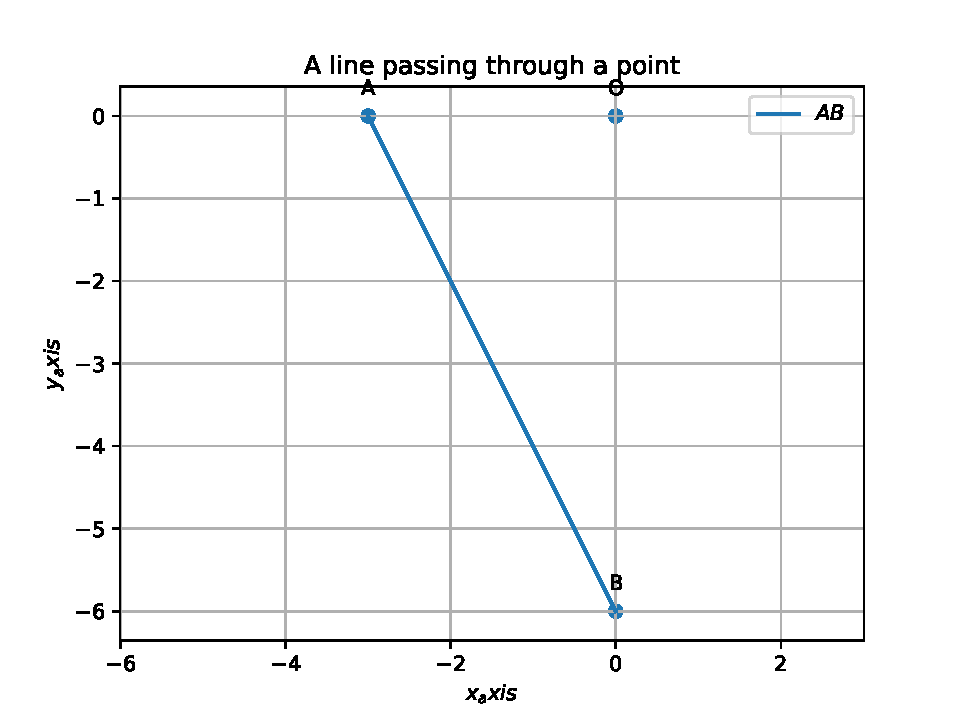
\includegraphics[width=\columnwidth]{chapters/11/10/2/5/figs/line1.pdf}
	\end{center}
\caption{}
\label{fig:chapters/11/10/2/5/Fig1}
\end{figure}

